\section{Introduction}
I have spent the majority of my time this week adding attention loss to my AMNet and testing it with features extracted by ResNet50.

So far I had just only worked with the Long-term subtask and I figured out that the Long-term Memory dataset was nothing but useless garbage. So till that moment I would start working with the Short-term subtask.

\section{AMNet}
\subsection{Attention Loss}
The model which I had used last week even though deployed the attention concept but I did not used the attention loss beside the normal Mean-squared error. So this week I tried to implement the attention loss in my network and hope it would perform better.


\subsection{Training on Dev-Set (extracted by ResNet50)}
\subsubsection{Strategy}
I used the same input strategy as the last week versions that I had trained. I splitted the provided Dev-Set for this challenge into three parts, since the Dev-Set had 8000 videos, I picked \textbf{\emph{6000}} videos for training, \textbf{\emph{1000}} videos for validating and the last \textbf{\emph{1000}} videos for testing.

\subsubsection{Version 2}
I kept the input size and hidden size as the same as the previous version that I had trained on Dev-Set last week. This times I changed the number of stacking LSTM layer to \textbf{\emph{1}} and the sequence length to \textbf{\emph{8}}. As mentioned above, I tried to conduct the same loss function as the one proposed by the authors which was a combination of mean squared error and attention penalty. There was one new hyper-parameter gamma which specified the impact of the attention penalty. I used its value of \textbf{\emph{1e-5}}. Finally was the ADAM optimizer with learning rate of \textbf{\emph{1e-4}}.

After \textbf{\emph{1000}} epochs I luckily got the loss decreasing but the correlation was not stable. My loss value was around \textbf{\emph{0.156}} and the best correlation value on validate set I got was only \textbf{\emph{0.23}}.

\newpage
\begin{figure}[!ht]
\centering
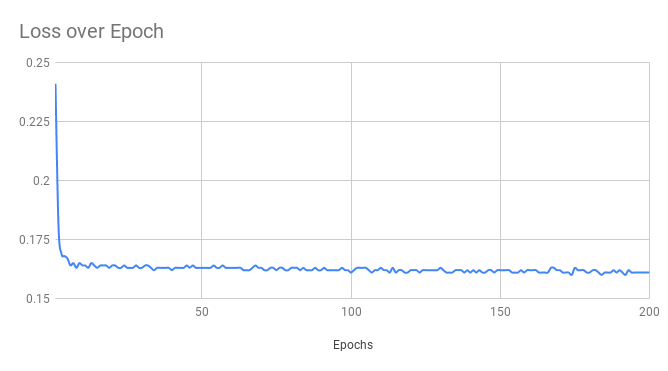
\includegraphics[width=\textwidth]{week13-amnet-devset-short-v2-loss.png}
\caption{Loss over Epoch (on Train set).}
\end{figure}

\begin{figure}[!ht]
\centering
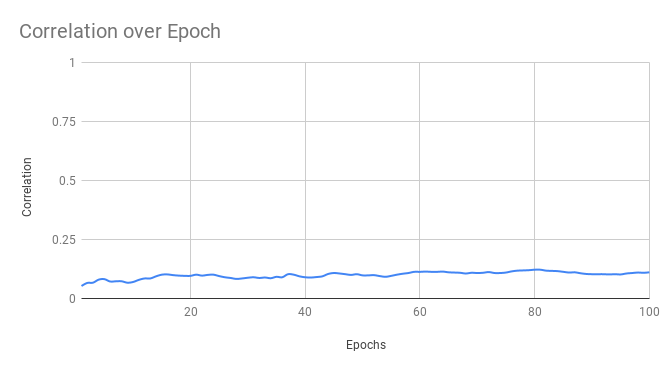
\includegraphics[width=\textwidth]{week13-amnet-devset-short-v2-correl.png}
\caption{Correlation over Epoch (on Validate set).}
\end{figure}

Lately, I used this pre-trained model to calculate the correlation value on the test, the correlation was a little bit lower, which was \textbf{\emph{0.18}}.

\section{Conclusion}
At this moment I started thinking that my extracted features were the problem. After testing my extracted features with my teammate Long-Short term memory network, my final conclusion was my ResNet50 extracted features were the problem causing my correlation horrible.
